%
\chapter{Metodolog\'ia}

En la presente Proyecto de Tesis se ha decidido usar la metodolog\'ia  CRISP-DM [10] ( Cross-industry standard process for data mining). Esta metodolog\'ia es ampliamente usada en miner\'ia de datos y es empleado por expertos en esta materia. \\

La metododolog\'a consiste en dividir el proceso de data minining en 6 fases las cuales se mencionan:



\begin{figure}[H]
\centering
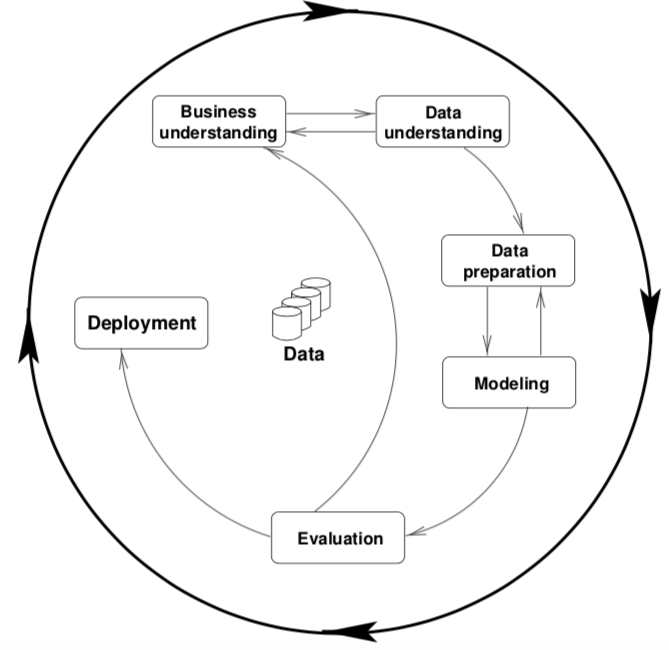
\includegraphics[scale=0.4]{chapters/img/Ch06_CRISP.PNG}
\caption{Fase del proceso de modelo CRISP-DM}
\end{figure}

\begin{itemize}
\item Entender el negocio
\item Entender los datos
\item Preparar los datos
\item Modelar
\item Evaluar
\item Desplegar
\end{itemize}


\section{Entender el negocio}

En este apartado se define que debemos conocer claramente el negocio sobre el cu\'as estamos analizando los datos

\section{Entender los datos}

Comprender la naturaleza del datos, identificando nuestra variables independientes, en este apartado es importante identificar la fuentes de los datos

\section{Preparar los datos}
Es un mecanismo donde aplicamos t\'ecnicas para mitigar los datos faltantes , son las conocidas como t\'ecnicas de clean data

\section{Modelar}
Con los datos listos para ser procesados, se realiza una an\'alisis descriptivo y elegimos un modelo de acuerdo a la naturaleza de los datos.  

\section{Evaluar}
Evaluamos los datos obtenidos por el modelo con los datos reales y verificamos si nuestro modelo es el correcto

\section{Desplegar}
Una vez obtenido el modelo m\'as parsimonioso procedemos al despliegue del modelo en un entorno productivo para su uso por los usuarios finales.


